% ==============================================================================
% SECCIÓN 7: DESCRIPCIÓN Y ARQUITECTURA DE LA SOLUCIÓN
% ==============================================================================
\newpage
\section{Descripción y Arquitectura de la Solución}

La visita al centro del 2 de octubre de 2026 se planteó para conocer los espacios, la dinámica de las clases, los apoyos existentes y la forma de trabajo con el alumnado (véase la sección de seguimiento). La documentación recoge estos ámbitos de observación, pero aún no concreta resultados particulares. Como respuesta provisional, se propone una agenda individual con actividades guiadas y apoyos configurables: organiza la secuencia de trabajo, facilita que el alumnado consulte qué debe hacer y permite registrar su avance sin imponer un único tipo de apoyo. La utilidad de estas decisiones deberá contrastarse con el centro y el alumnado mediante la revisión del prototipo y pruebas de uso.

La arquitectura tecnológica se plantea como hipótesis de implementación, no como conclusión de la observación. La elección de dispositivos, alojamiento, seguridad y mantenimiento queda pendiente de validación con el centro.

\subsection{Esquema lógico}
\noindent\figuracambiada{cambioArquitectura}{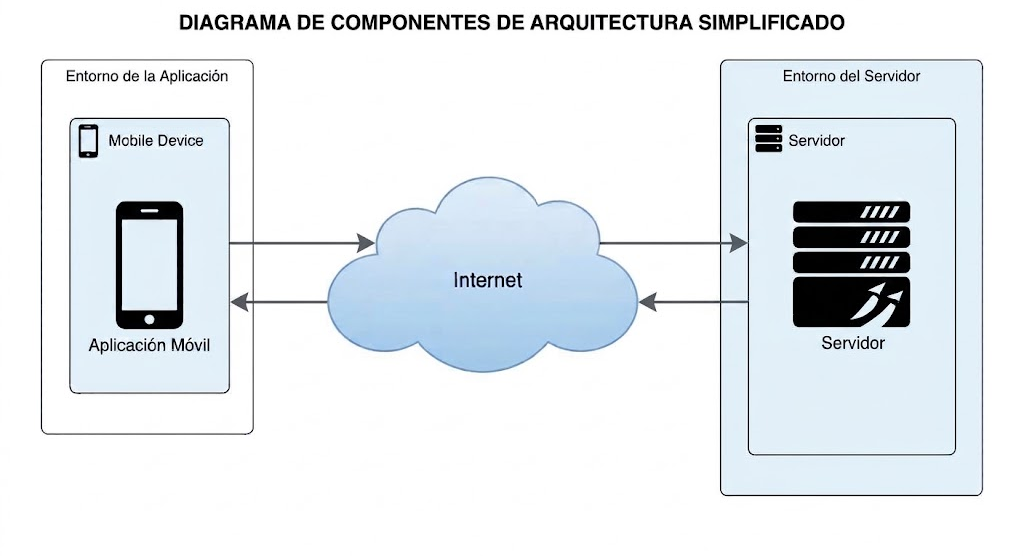
\includegraphics[width=\dimexpr\textwidth-2\fboxrule\relax,height=0.75\textheight,keepaspectratio]{images/arquitectura.png}}

\subsection{Flujo principal}
Las decisiones funcionales responden al contexto de uso observado y se concretan en los requisitos verificables:

\begin{enumerate}[leftmargin=*]
  \item \textbf{Acceso y responsabilidades.} Cada perfil accede solo a las funciones y datos que le corresponden; el administrador gestiona las cuentas y asociaciones. Así se separan las responsabilidades del alumnado, el personal y los tutores. (\hyperlink{rf-01}{RF-01}--\hyperlink{rf-06}{RF-06}; \hyperlink{rnf-03}{RNF-03})

  \item \textbf{Planificación.} El personal asigna actividades durante el horario escolar y los tutores autorizados, fuera de él; el personal también puede asignar rutinas existentes. El alumnado puede añadir actividades personales, diferenciadas de las asignadas. Esta división refleja los distintos roles de apoyo contemplados en los requisitos. (\hyperlink{rf-07}{RF-07}, \hyperlink{rf-10}{RF-10}, \hyperlink{rf-12}{RF-12}, \hyperlink{rf-17}{RF-17}--\hyperlink{rf-19}{RF-19})

  \item \textbf{Consulta accesible.} El alumnado consulta las actividades por fecha y hora, y recibe instrucciones ordenadas con los apoyos configurados para su perfil. La agenda estructurada y los apoyos seleccionables son una respuesta a la necesidad de adaptar la interacción a la dinámica y diversidad del aula; su formato concreto se validará con usuarios. (\hyperlink{rf-20}{RF-20}--\hyperlink{rf-23}{RF-23}; \hyperlink{rnf-01}{RNF-01}, \hyperlink{rnf-05}{RNF-05}, \hyperlink{rnf-06}{RNF-06})

  \item \textbf{Realización y continuidad.} El alumnado completa las instrucciones paso a paso y consulta el progreso; el temporizador acompaña la actividad. Si no hay conexión, conserva el acceso a las actividades sincronizadas y registra el avance para sincronizarlo después. Estas funciones buscan apoyar el seguimiento sin depender de la supervisión continua del personal, sujeto a validación de uso. (\hyperlink{rf-24}{RF-24}--\hyperlink{rf-29}{RF-29}; \hyperlink{rnf-04}{RNF-04}, \hyperlink{rnf-07}{RNF-07})

\end{enumerate}
